\documentclass[9pt, technote]{article}
\usepackage{eadca-template}
\usepackage[plain]{algorithm}

\usepackage[brazil]{babel}
\usepackage[utf8]{inputenc}
\usepackage[T1]{fontenc}

\usepackage{graphicx,url}
\usepackage[hang]{subfigure}
\usepackage{psfrag}

\usepackage{siunitx}
\usepackage{mathtools}
\usepackage{booktabs}
\usepackage{pbox}
\usepackage{etoolbox}
\graphicspath{{../figures/}}

\newcommand{\sigmoid}{\text{Sigmoid}}
\newcommand{\sen}{\text{sen}}
\newcommand{\selu}{\text{SELU}}
\newcommand{\relu}{\text{ReLU}}
\newcommand{\elu}{\text{ELU}}
\newcommand{\lecun}{\text{Lecun}}
\newcommand{\he}{\text{He}}
\newcommand{\glorot}{\text{Glorot}}
\newcommand{\normal}{\text{Normal}}
\newcommand{\uniform}{\text{Uniforme}}

\sloppy

\title{{\noindent 
\includegraphics[scale = 0.5]{banner-grande.png}}\\ Predição de Séries Temporais Baseada em Redes Neurais
Artificiais}

\author{Aluno: João Pedro de Oliveira Pagnan [FEEC/UNICAMP]\\Orientador: Prof.  Levy Boccato [FEEC/UNICAMP]\\
Coorientador: Prof. Romis Ribeiro de Faissol Attux [FEEC/UNICAMP]}

\address{Departamento de Engenharia de Computação e Automação Industrial (DCA)\\ Faculdade de Engenharia Elétrica e de Computação (FEEC) \\
  Universidade Estadual de Campinas (UNICAMP)}

\hyphenation{}
\pagestyle{fancy}

\begin{document}

\twocolumn[
\maketitle
\thispagestyle{fancy}
  \keywords{Redes Neurais Artificiais, Sistemas Caóticos, Séries Temporais}
\hrule
]

\section{Introdução}

A predição de séries temporais é uma das aplicações mais interessantes do tratamento de informação. O desafio de antecipar padrões de comportamento e construir modelos que sejam apropriados para explicar determinados fenômenos da natureza tem importância  para a biologia, economia, automação industrial, meteorologia e diversas outras áreas da ciência \cite{box2015time}.

Na literatura, encontramos diversos tipos de modelos para a  predição de séries temporais, desde métodos clássicos lineares, como o modelo autorregressivo (AR) \cite{box2015time} até métodos não-lineares utilizando, por exemplo, redes neurais artificiais, sendo que dessas se destacam as redes do tipo \textit{Multilayer Perceptron} (MLP) \cite{rosenblatt1958perceptron} e as redes recorrentes, especialmente a \textit{Long Short-Term Memory} (LSTM)  \cite{connor1994recurrent} e a \textit{Echo State Network} (ESN) \cite{jaeger2007echo}.

Uma classe de sistemas dinâmicos particularmente relevante dentro do contexto de modelagem e predição de séries temporais está ligada à ideia de dinâmica caótica. Diversos fenômenos naturais, como a dinâmica populacional de uma espécie, a dinâmica atmosférica de uma região, ou até mesmo as órbitas de um sistema com três ou mais corpos celestes podem exibir comportamento caótico. Apesar de serem determinísticos (e, portanto, previsíveis), esses sistemas são extremamente sensíveis às condições iniciais \cite{fiedler1994caos}. Isso causa um problema para a predição das séries temporais originadas por eles, pois uma pequena incerteza na medida afetará toda a previsão. 

Tendo em vista o desempenho de modelos não-lineares para previsão de diversas séries temporais \cite{connor1994recurrent}, optamos por estudar a aplicabilidade de redes neurais artificiais à previsão de séries relacionadas a sistemas com dinâmica caótica.

Esta pesquisa comparou o desempenho de quatro arquiteturas distintas de redes neurais artificiais: a rede \textit{Multilayer Perceptron} \cite{rosenblatt1958perceptron}, a rede \textit{Long Short-Term Memory} \cite{connor1994recurrent}, a rede \textit{Gated Recurrent Unit} (GRU) \cite{cho2014learning} e, por fim, a rede \textit{Echo State Network} (ESN) \cite{jaeger2007echo}.

A comparação foi realizada em quatro cenários de sistemas caóticos, sendo dois destes a tempo discreto e dois a tempo contínuo. No caso, os sistemas a tempo discreto foram as séries temporais do mapa de Hénon \cite{henon1976two}, e a série temporal relacionada ao mapa logístico \cite{may1976simple}. Já os sistemas a tempo contínuo foram o sistema de Lorenz \cite{lorenz1963deterministic} e as equações de Mackey-Glass \cite{mackey1977oscillation}. Nos sistemas multidimensionais, como o mapa de Hénon e o sistema de Lorenz, foi utilizada a série temporal em $\hat{x}$.

Iniciamos a análise através de um processo de \textit{gridsearch} para determinarmos os parâmetros ótimos para as redes neurais em cada cenário. Em seguida, utilizando os melhores parâmetros, realizou-se um estudo da progressão erro quadrático médio (EQM) com o número de amostras de entrada do modelo preditor (nesse caso, chamado de $K$). Por fim, comparamos qual foi a média e o desvio padrão do EQM com o melhor valor de $K$ de cada modelo nos quatro cenários.

Através desta pesquisa, percebe-se que a ESN possui o melhor desempenho dentre todos os modelos, em todos os cenários. As redes \textit{Echo State Network} têm a vantagem de necessitarem de bem menos recursos computacionais do que os outros modelos avaliados, obtendo um desempenho consideravelmente superior mesmo com um tempo de treinamento ínfimo se comparado às redes neurais artificiais tradicionais.

\section{Metodologia}

\subsection{Geração de dados}

Como o intuito do projeto é analisar o desempenho dos modelos preditores citados em sistemas caóticos, os dados necessários para o treinamento e para a análise da \textit{performance} podem serem obtidos através da solução numérica dos sistemas caóticos. As próximas seções evidenciam o processo utilizado, junto com os parâmetros escolhidos para os sistemas caóticos.

\subsubsection{Mapa de Hénon}

O mapa de Hénon foi um dos sistemas a tempo discreto escolhidos para esta pesquisa. Esse sistema foi proposto por Michel Hénon em 1976 como um modelo simplificado de uma seção de Poincaré do atrator de Lorenz, sendo descrito pelas equações abaixo \cite{henon1976two}:
\begin{subequations}
\begin{equation}
x[n+1] = y[n] + 1 - a\cdot (x[n])^2
\end{equation}
\begin{equation}
y[n+1] = b \cdot x[n]
\end{equation}
\end{subequations}

Para esta pesquisa, foram utilizados os valores usuais para os parâmetros $a$ e $b$. Logo, têm-se que $a = 1.4$ e $b = 0.3$. Além disso, neste e nos outros sistemas, foi gerado um conjunto de $5000$ dados. As figuras a seguir mostram a série temporal em $\hat{x}$ e o atrator obtido com a simulação:
\begin{figure}[H]
     \centering
     \begin{subfigure}
         \centering
         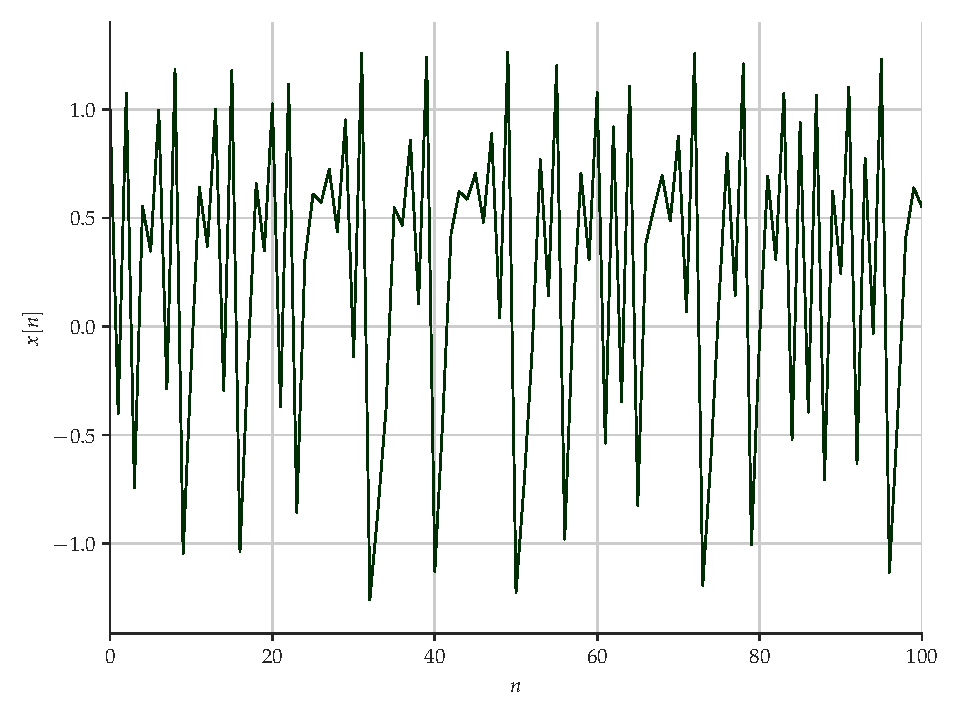
\includegraphics[scale=0.24]{serie-henon-x.pdf}
         %\caption{$y=5/x$}
     \end{subfigure}
     \begin{subfigure}
         \centering
         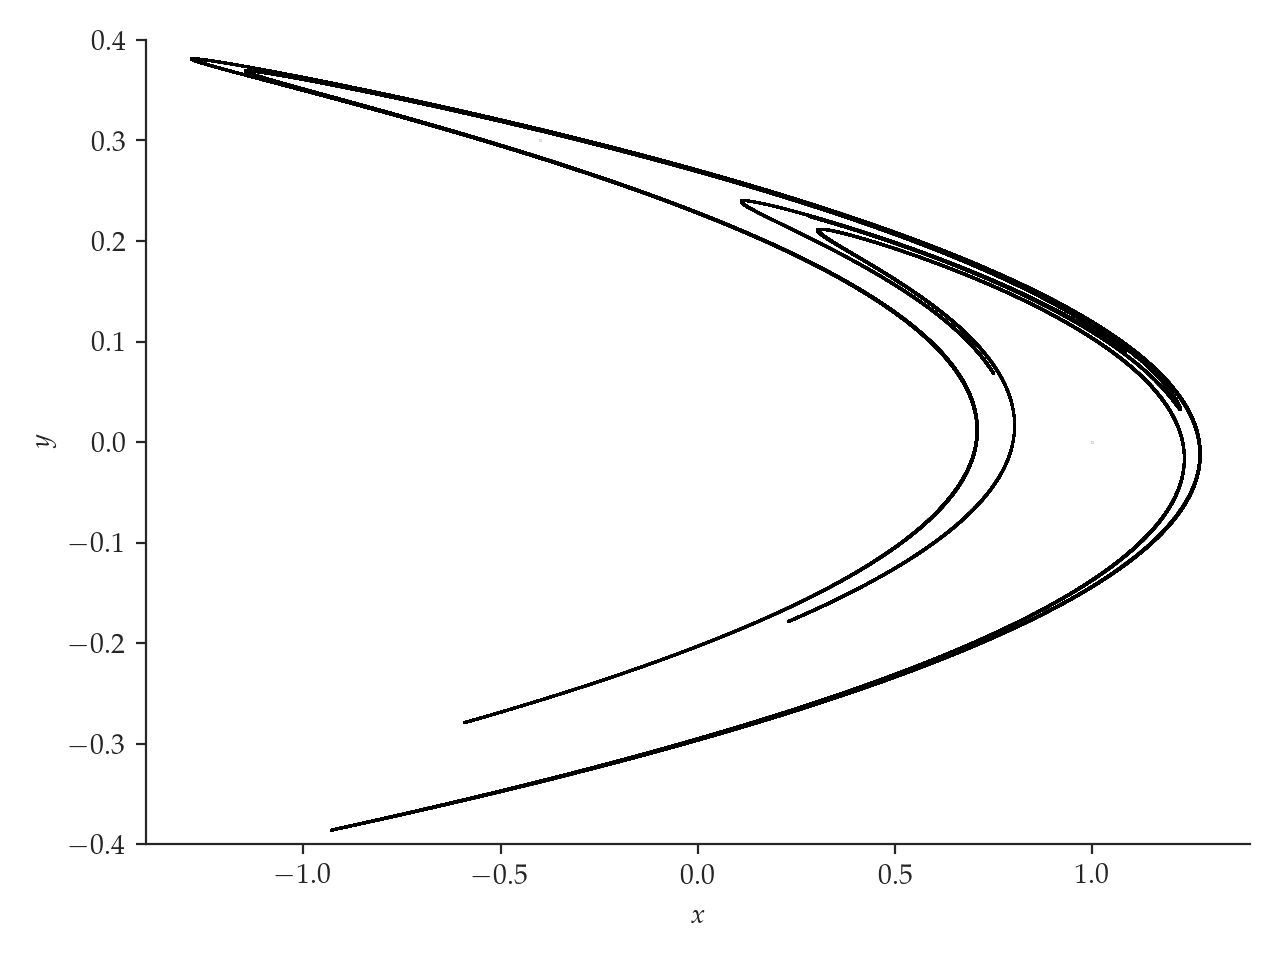
\includegraphics[scale=0.24]{mapa-de-henon.png}
         %\caption{$y=x$}
     \end{subfigure}
     \caption{À esquerda, as cem primeiras iterações da série temporal em $\hat{x}$ do mapa de Hénon e, à direita, o atrator correspondente à simulação}
     \label{fig:henon}
\end{figure}

\subsubsection{Mapa logístico}

Conforme foi dito anteriormente, o outro sistema caótico a tempo discreto simulado foi o mapa logístico. Descrito em 1976 por Robert May, o mapa logístico é uma das formas de modelar a população de uma determinada espécie em certos instantes de tempo \cite{may1976simple}. A equação de diferenças que descreve esse sistema pode ser vista abaixo:
\begin{equation}\label{eq:logistic}
x[n+1] = r\cdot x[n] \cdot (1 - x[n])
\end{equation}

Nesse caso, o sistema não chega a operar em caos para qualquer valor de $r$. Assim, como o estudo visa analisar o desempenho para sistemas caóticos, foi utilizado $r=3.86$, que, conforme será visto no diagrama de bifurcação abaixo, faz com que a série temporal dada pela equação (\ref{eq:logistic}) opere em caos. Novamente, foram simuladas $5000$ iterações:
\begin{figure}[H]
     \centering
     \begin{subfigure}
         \centering
         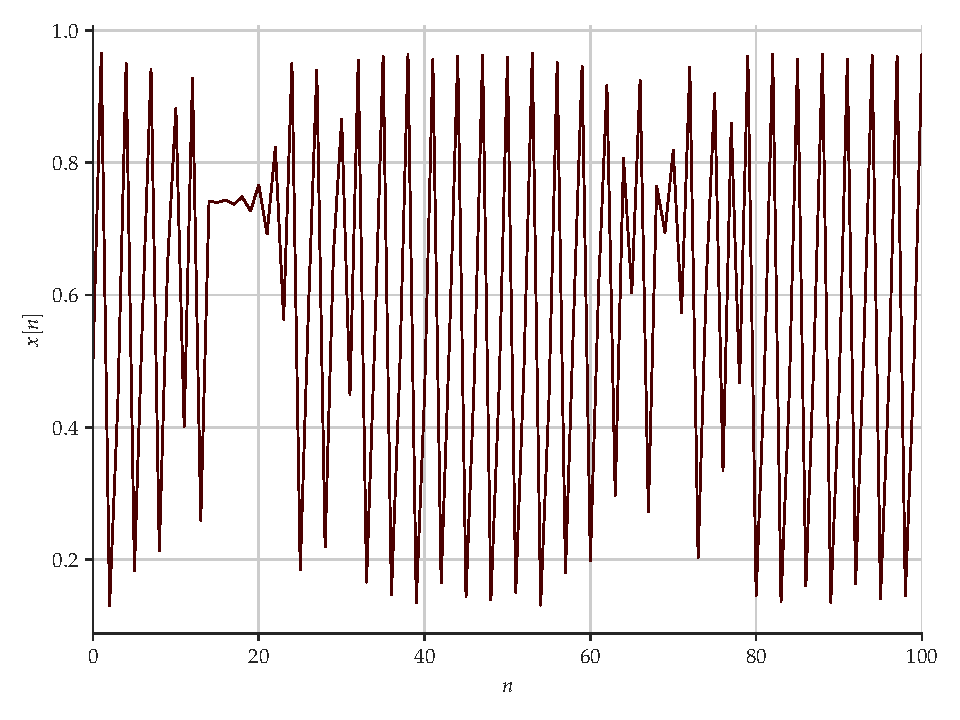
\includegraphics[scale=0.24]{serie-logistico.pdf}
         %\caption{$y=5/x$}
     \end{subfigure}
     \begin{subfigure}
         \centering
         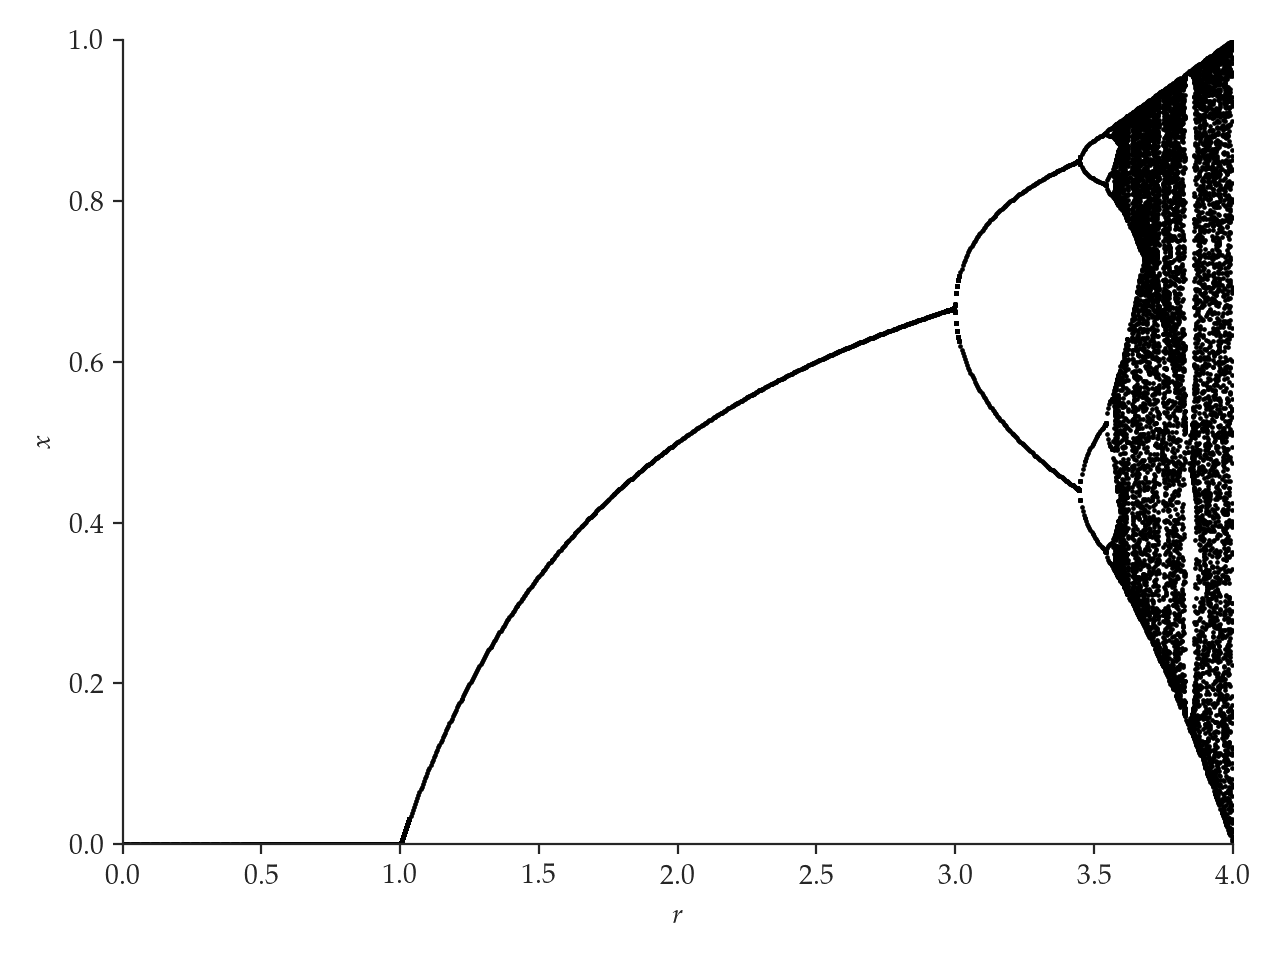
\includegraphics[scale=0.24]{mapa-logistico.png}
         %\caption{$y=x$}
     \end{subfigure}
     \caption{À esquerda, as cem primeiras iterações da série temporal do mapa logístico e, à direita, o diagrama de bifurcação este sistema}
     \label{fig:logistic}
\end{figure}

\subsubsection{Sistema de Lorenz}

O sistema de Lorenz foi um dos sistemas dinâmicos caóticos a tempo contínuo simulados nessa pesquisa. Este sistema foi um dos primeiros grandes trabalhos de sistemas caóticos, sendo considerado por muitos a pesquisa que inaugurou a área \cite{gleick1998chaos}. Lorenz modela, através de três equações diferenciais, o fluxo de um fluído em um volume uniformemente aquecido na camada inferior, e uniformemente resfriado na camada superior \cite{lorenz1963deterministic}:
\begin{subequations}
\begin{equation}
\frac{dx}{dt} = -\sigma \cdot (x - y)
\end{equation}
\begin{equation}
\frac{dy}{dt} = x \cdot (\rho - z) - y
\end{equation}
\begin{equation}
\frac{dz}{dt} = x \cdot y - \beta \cdot z
\end{equation}
\end{subequations}

Para a simulação numérica foi considerado que $\sigma = 10$, $\beta = \frac{8}{3}$, $\rho = 28$ e foi utilizado $dt = 0.01$, gerando $5000$ dados, assim como nos casos discretos. As figuras abaixo mostram a série temporal em $\hat{x}$ e o atrator de Lorenz para a condição inicial $[x(0)\; y(0)\; z(0)]^T = [0.1\; 0\; 0]^T$:
\begin{figure}[H]
     \centering
     \begin{subfigure}
         \centering
         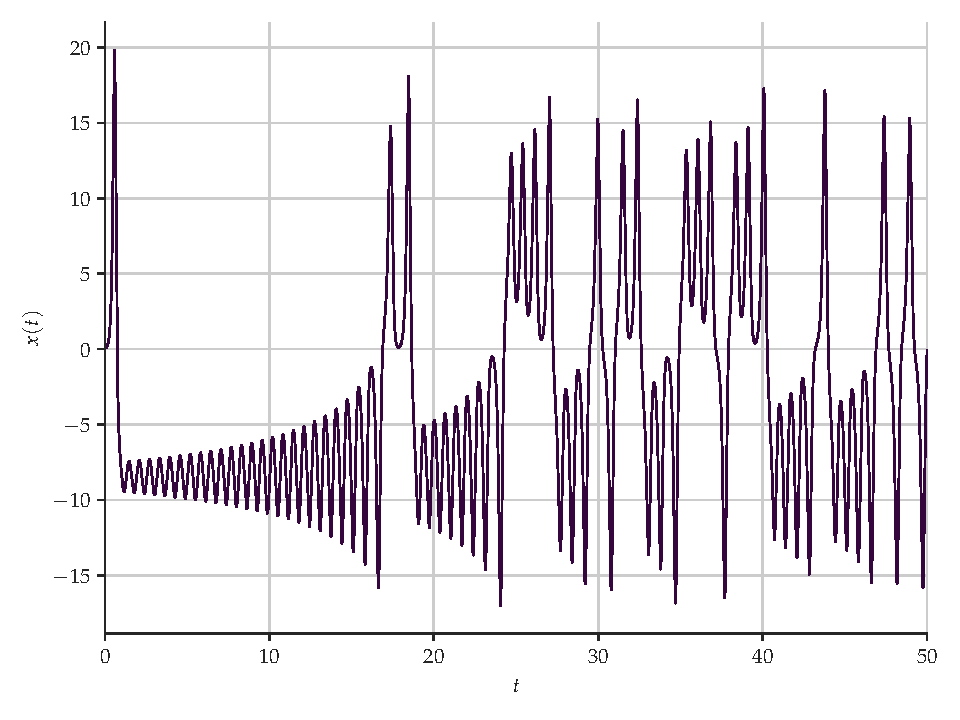
\includegraphics[scale=0.24]{serie-lorenz-x.pdf}
         %\caption{$y=5/x$}
     \end{subfigure}
     \begin{subfigure}
         \centering
         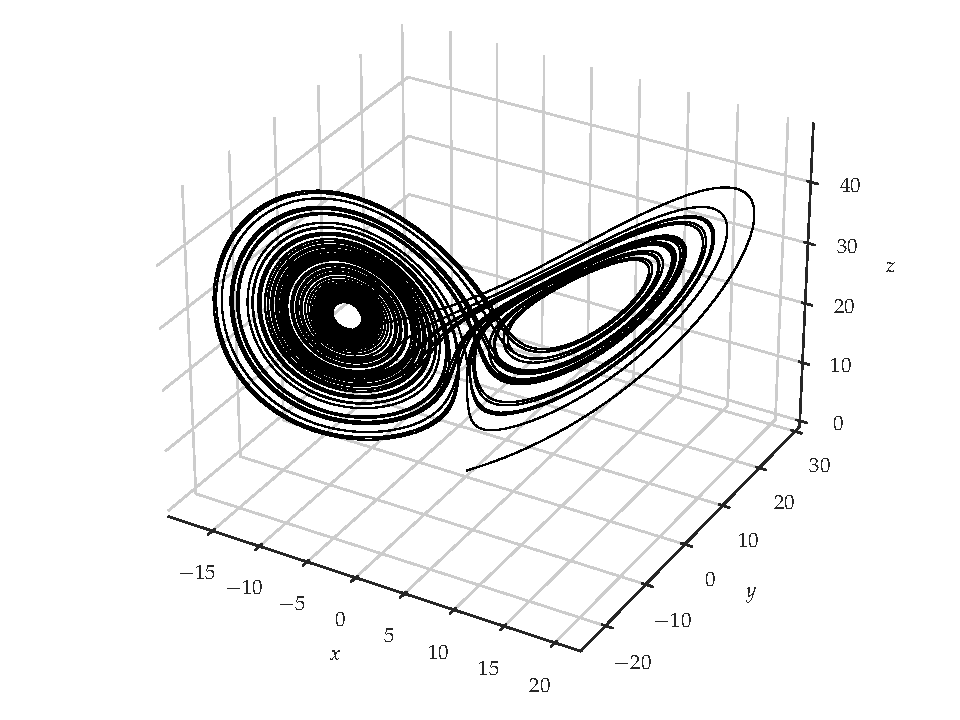
\includegraphics[scale=0.24]{diagrama-de-fases-lorenz.pdf}
         %\caption{$y=x$}
     \end{subfigure}
     \caption{À esquerda, a série temporal em $\hat{x}$ do sistema de Lorenz simulado e, à direita, o diagrama de fases correspondente à simulação}
     \label{fig:lorenz}
\end{figure}

\subsubsection{Equações de Mackey-Glass}

Por fim, o último sistema caótico simulado, este também a tempo contínuo, foram as equações de Mackey-Glass. Essas equações diferenciais com atraso temporal modelam o controle hormonal da produção de células brancas do sangue e podem serem vistas abaixo \cite{mackey1977oscillation}:
\begin{subequations}
\begin{equation}
\frac{dP(t)}{dt} = \frac{\beta_0\cdot \theta^n}{\theta^n + P(t - \tau)^n} - \gamma\cdot P(t)
\end{equation}
\begin{equation}\label{eq:mackey-glass-chaos}
\frac{dP(t)}{dt} = \frac{\beta_0\cdot \theta^n \cdot P(t - \tau)}{\theta^n + P(t - \tau)^n} - \gamma\cdot P(t)
\end{equation}
\end{subequations}

Neste caso, a equação (\ref{eq:mackey-glass-chaos}) exibe um comportamente caótico para valores mais altos de $\tau$. Para a simulação numérica, foi utilizado $n = 10$, $\gamma = 0.1$, $\beta = 0.2$, $\theta = 1$, $\tau = 22$ e $dt = 1.0$, gerando novamente $5000$ dados, resultando na seguinte série temporal e no seguinte atrator:
\begin{figure}[H]
     \centering
     \begin{subfigure}
         \centering
         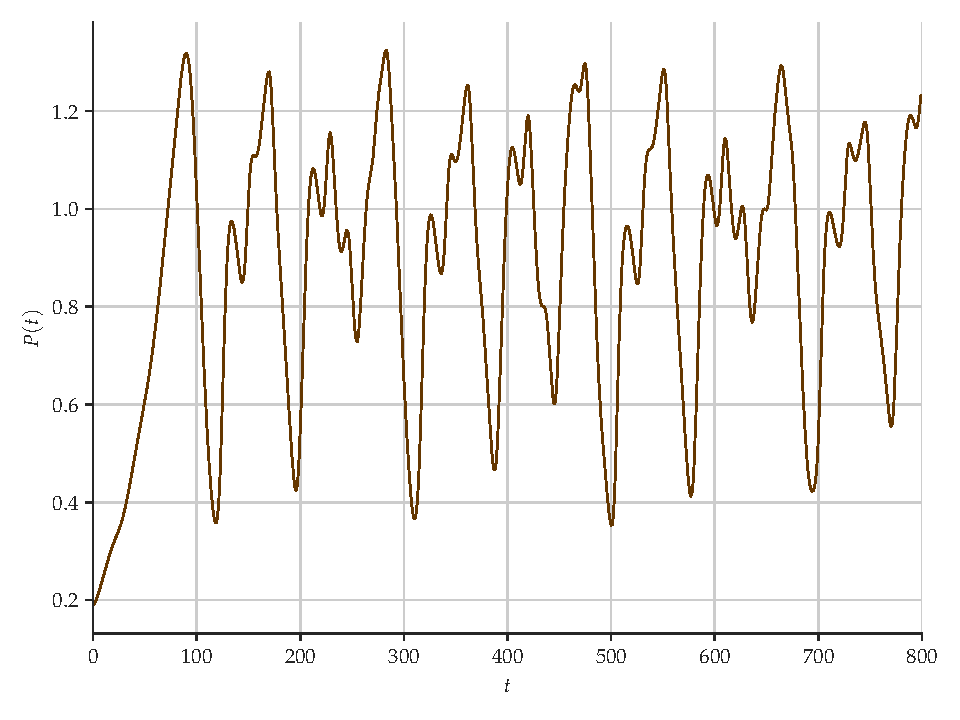
\includegraphics[scale=0.24]{serie-mackeyglass.pdf}
         %\caption{$y=5/x$}
     \end{subfigure}
     \begin{subfigure}
         \centering
         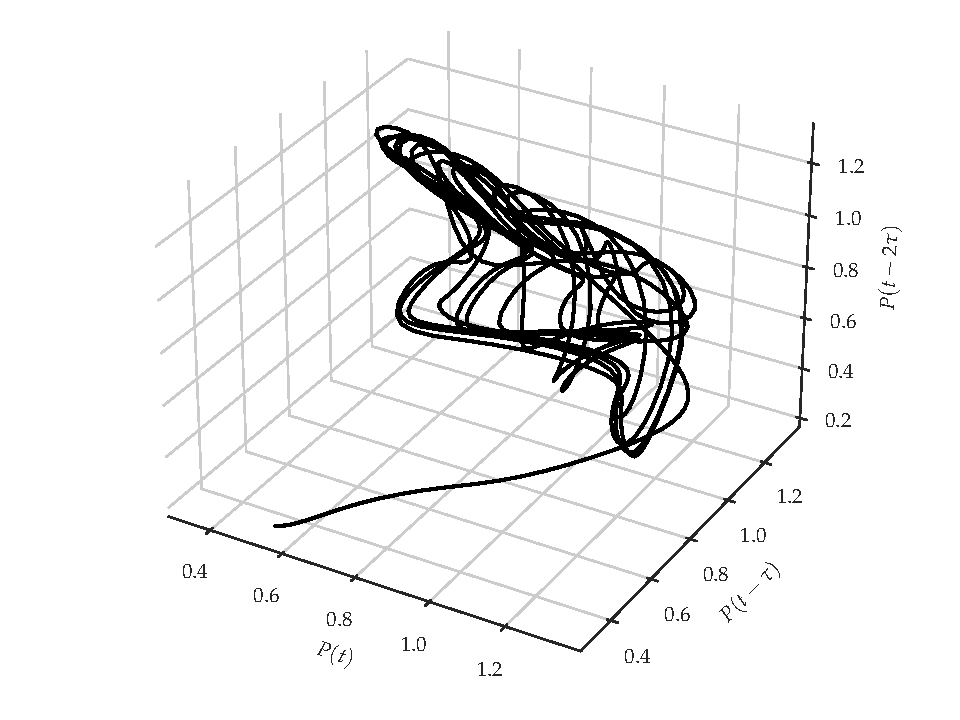
\includegraphics[scale=0.24]{atrator-mackeyglass.pdf}
         %\caption{$y=x$}
     \end{subfigure}
     \caption{À esquerda, a série temporal da equação (\ref{eq:mackey-glass-chaos}) exibida de $t = 0 $ a $t = 800$ e, à direita, o atrator correspondente à simulação}
     \label{fig:mackey-glass}
\end{figure}

\subsection{Obtenção dos melhores parâmetros}

\BeforeBeginEnvironment{tabular}{\tiny}

Como foi mencionado na seção introdutória, foi realizado um procedimento de \textit{gridsearch} para a determinação dos melhores parâmetros para as redes neurais. Nesse caso, cada arquitetura testou parâmetros diferentes nesse processo, logo, as próximas seções indicam o que foi testado para cada modelo. Vale reforçar que o \textit{gridsearch} foi realizado em todos os cenários de sistemas caóticos analisados, de forma a obter os melhores parâmetros para cada um deles.

\subsubsection{MLP}

Para as redes \textit{Multilayer Perceptron}, foi testado o tamanho do \textit{batch} para o treinamento ($2$, $4$, $8$, $16$, $32$), se será ou não utilizado uma camada de \textit{batch normalization}, a função de ativação para os neurônios \textit{Perceptron} na camada intermediária ($\selu$, $\relu$, $\elu$, $\tanh$, $\sigmoid$), a inicialização dos pesos dos neurônios ($\glorot$, $\he$, $\lecun$, tanto com distribuição normal, quanto uniforme), o número de neurônios na camada intermediária ($5$, $10$, $15$, $20$, $30$, $50$, $75$, $100$) e, por fim, a taxa de aprendizagem ($0.001$, $0.003$, $0.005$, $0.008$, $0.01$). 

O \textit{gridsearch} utilizou validação cruzada com $4$ \textit{folds} nos dados de treinamento, que correspondiam a $85\%$ dos primeiros dados das séries temporais, isto é, os primeiros $4250$ valores. Essa proporção entre os dados de treinamento e de teste foi utilizada para todas as redes analisadas.

Vale reforçar que foi utilizada apenas uma camada intermediária em cada cenário. As melhores configurações obtidas podem serem vistas na tabela abaixo:
\begin{table}[!ht]
\begin{center}
\begin{tabular}{c c c c c c c}
  \textbf{Cenário}  & \pbox{0.85cm}{\centering \textbf{\; \, \textit{Batch\newline normalization}}} & \pbox{0.4cm}{\centering \textbf{\textit{Batch size}}} & \pbox{0.65cm}{\centering \textbf{Função de ativação}} & \pbox{0.9cm}{\centering \textbf{Inicialização}} & \pbox{0.745cm}{\centering \textbf{Nº de neurônios}} & \pbox{1cm}{\centering \textbf{\, Taxa de\newline aprendizagem}}\\
 \hline
 \addlinespace
 \pbox{0.7cm}{\centering \textbf{Mapa de\newline Hénon}} & Não & $8$ & $\sigmoid$ & $\glorot\, \normal$ & $50$ & $0.003$\\  
  \addlinespace
 \pbox{0.7cm}{\centering \textbf{Mapa\newline logístico}} & Não & $2$ & $\tanh$ & $\glorot\, \uniform$ & $10$ & $0.003$\\ 
  \addlinespace
 \pbox{0.9cm}{\centering \textbf{Sistema de\newline Lorenz}} & Não & $2$ & $\selu$ & $\lecun\, \normal$ & $50$ & $0.001$\\ 
  \addlinespace
 \pbox{0.929cm}{\centering \textbf{Equações de\newline Mackey-Glass}} & Não & $4$ & $\tanh$ & $\glorot\, \normal$ & $5$ & $0.001$\\ 
\end{tabular}
\caption{Melhores parâmetros para a rede MLP nos cenários em análise}
\end{center}
\end{table}

\subsubsection{LSTM e GRU}

O processo para a LSTM e GRU foram bem similares, considerando que essas arquiteturas de redes neurais são semelhantes. A principal diferença com relação ao \textit{gridsearch} da MLP foi o fato de que, ao invés de utilizar-se validação cruzada com $k-$\textit{folds}, foi utilizado \textit{holdout}. Esse processo dividiu o conjunto de treinamento (novamente composto por $85\%$ dos dados gerados) em $4$ seções. Cada seção era composta por uma fração dos dados de treinamento, sendo que cada seção incluia a seção anterior no seu conjunto de dados.

Por exemplo, a segunda seção obtida pelo \textit{holdout} inclui a primeira seção e mais alguns dados, além de uma subdivisão de validação que será utilizada para avaliar o resultado. Com isso, obtém-se conjuntos sequenciais de dados para avaliação do desempenho. Esse procedimento é necessário para as redes recorrentes pois a relação temporal entre os dados de entrada deve ser levada em conta.

Foi avaliado o \textit{batch size} ($2$, $4$, $8$, $16$, $32$), a inicialização dos pesos ($\glorot \, \uniform$, $\glorot \, \normal$), o número de neurônios recorrentes na camada intermediária ($5$, $10$, $15$, $20$, $30$, $50$, $75$, $100$), e a taxa de aprendizagem ($0.001$, $0.003$, $0.005$, $0.008$, $0.01$), novamente utilizando apenas uma camada intermediária. Vale reforçar que a função de ativação usual da célula recorrente não foi alterada ($\tanh$), assim, para o sistema de Lorenz, foi feito um ajuste de escala para evitar a saturação na saída dos neurônios.

Os resultados obtidos para a LSTM e para a GRU podem serem vistos nas tabelas a seguir:
\begin{table}[!ht]
\begin{center}
\begin{tabular}{c c c c c}
  \textbf{Cenário} & \pbox{0.4cm}{\centering \textbf{\textit{Batch size}}} & \pbox{0.9cm}{\centering \textbf{Inicialização}} & \pbox{0.745cm}{\centering \textbf{Nº de neurônios}} & \pbox{1cm}{\centering \textbf{\, Taxa de\newline aprendizagem}}\\
 \hline
 \addlinespace
 \pbox{0.7cm}{\centering \textbf{Mapa de\newline Hénon}} & $4$ & $\glorot\, \normal$ & $15$ & $0.005$\\  
  \addlinespace
 \pbox{0.7cm}{\centering \textbf{Mapa\newline logístico}} & $2$ & $\glorot\, \uniform$ & $100$ & $0.008$\\ 
  \addlinespace
 \pbox{0.9cm}{\centering \textbf{Sistema de\newline Lorenz}} & $4$ & $\glorot\, \uniform$ & $15$ & $0.003$\\ 
  \addlinespace
 \pbox{0.929cm}{\centering \textbf{Equações de\newline Mackey-Glass}} & $2$ & $\glorot\, \uniform$ & $50$ & $0.003$\\ 
\end{tabular}
\caption{Melhores parâmetros para a rede LSTM nos cenários em análise}
\end{center}
\end{table}

\begin{table}[!ht]
\begin{center}
\begin{tabular}{c c c c c}
  \textbf{Cenário} & \pbox{0.4cm}{\centering \textbf{\textit{Batch size}}} & \pbox{0.9cm}{\centering \textbf{Inicialização}} & \pbox{0.745cm}{\centering \textbf{Nº de neurônios}} & \pbox{1cm}{\centering \textbf{\, Taxa de\newline aprendizagem}}\\
 \hline
 \addlinespace
 \pbox{0.7cm}{\centering \textbf{Mapa de\newline Hénon}} & $4$ & $\glorot\, \normal$ & $30$ & $0.003$\\  
  \addlinespace
 \pbox{0.7cm}{\centering \textbf{Mapa\newline logístico}} & $2$ & $\glorot\, \normal$ & $100$ & $0.003$\\ 
  \addlinespace
 \pbox{0.9cm}{\centering \textbf{Sistema de\newline Lorenz}} & $8$ & $\glorot\, \uniform$ & $30$ & $0.001$\\ 
  \addlinespace
 \pbox{0.929cm}{\centering \textbf{Equações de\newline Mackey-Glass}} & $2$ & $\glorot\, \uniform$ & $10$ & $0.005$\\ 
\end{tabular}
\caption{Melhores parâmetros para a rede GRU nos cenários em análise}
\end{center}
\end{table}

\subsubsection{ESN}

A \textit{Echo State Network} foi a rede neural mais distinta das outras analisadas nesta pesquisa. Essa rede recorrente baseia-se na teoria de computação por reservatório, chamada assim pois ela utiliza um reservatório de comportamentos dinâmicos que, ao serem combinados linearmente nos neurônios da camada de leitura, produzem as saídas da rede \cite{boccato2013novas}. 

O grande diferencial prático desta rede é que os pesos dos neurônios do reservatório são ajustados com valores fixos antes do treinamento da camada de saída. Esses valores são obtidos aleatoriamente, seguindo determinados parâmetros, como o raio espectral que determina o maior valor singular da matriz de pesos do reservatório,  a taxa de vazamento que representa a velocidade com a qual o reservatório atualiza suas dinâmicas. Além disso, normalmente, a matriz dos pesos do reservatório é esparsa \cite{jaeger2007echo}.

Devido a isso, o ajuste dos neurônios na camada de leitura pode ser realizado com um procedimento de regressão linear, sem necessitar de um treinamento iterativo, como nas redes anteriores. Esse fato economiza tempo de processamento e garante que será atingido o mínimo global da função custo utilizada.

Logo, para esta rede foi realizado um \textit{gridsearch} para determinar o número de neurônios na camada de leitura ($30$, $50$, $70$, $90$, $100$, $120$, $140$, $160$, $180$, $200$, $240$, $280$, $320$, $360$, $400$, $440$, $480$, $500$) e o valor para o raio espectral ($0.1$, $0.2$, $0.3$, $0.4$, $0.5$, $0.6$, $0.7$, $0.8$, $0.9$, $0.95$, $0.96$, $0.97$, $0.98$, $0.99$) e, por tratar-se de uma rede recorrente, também foi utilizado o processo de \textit{holdout} descrito na seção anterior. Vale também mencionar que a taxa de vazamento foi fixada em $0.9$ para todos os cenários.

Obteve-se assim, as seguintes configurações para a ESN em cada um dos cenários:
\begin{table}[!ht]
\begin{center}
\begin{tabular}{c c c}
  \textbf{Cenário} & {\centering \textbf{Raio espectral}} & {\centering \textbf{Nº de neurônios}}\\
 \hline
 \addlinespace
 \pbox{0.7cm}{\centering \textbf{Mapa de\newline Hénon}} & $0.1$ & $500$\\  
  \addlinespace
 \pbox{0.7cm}{\centering \textbf{Mapa\newline logístico}} & $0.1$ & $500$\\ 
  \addlinespace
 \pbox{0.9cm}{\centering \textbf{Sistema de\newline Lorenz}} & $0.2$ & $120$\\ 
  \addlinespace
 \pbox{0.929cm}{\centering \textbf{Equações de\newline Mackey-Glass}} & $0.4$ & $500$\\ 
\end{tabular}
\caption{Melhores parâmetros para a rede ESN nos cenários em análise}
\end{center}
\end{table}

\subsection{Análise do melhor valor para $K$}

Com as melhores configurações para cada rede e cenário obtidas, foi analisada a progressão do erro quadrático médio para cada valor de $K$ para cada rede neural, em cada cenário. Para tal, cada rede (com as configurações ótimas) foi treinada utilizando $85\%$ dos dados gerados, sendo que $10\%$ dos dados de treinamento foi utilizado como o conjunto de validação (nas redes MLP, LSTM e GRU). Em seguida, com o modelo treinado, foi avaliado o EQM no conjunto de teste (que corresponde aos últimos $750$ dados). Esse processo foi realizado $5$ vezes para cada $K$, obtendo assim um valor médio e desvio-padrão para cada $K$ em cada cenário, para cada modelo.

Vale reforçar que, como o ajuste de parâmetros da ESN possui solução em forma fechada, não foi necessário utilizar um conjunto de validação no treinamento. No caso da MLP, LSTM e GRU, o processo iterativo de ajuste dos pesos utilizou um conjunto de validação de forma a seguir o procedimento de \textit{early stopping} para evitar o sobreajuste da rede.

As imagens abaixo mostram a progressão do EQM para cada $K$ obtida em todos os cenários para todas as redes:

\section{Resultados}

\section{Conclusões}

\bibliographystyle{ieeetr}
{\footnotesize
\bibliography{bib}
}
\pdfinfo{
  /Title  (Congresso PIBIC 2021 - João P. Pagnan)
  /CreationDate (D:20040502195600)
}


\end{document}